\section{Operational oceanography}
\label{S:operational_oceanography}

Mesoscale ocean prediction moved into operations across the early 2000s in a manner that lagged and imitated the path of NWP \citep{Harper:2008ub}. Operational oceanography is `big science' \citep{Petersen:2012tr} in the sense that it fundamentally relies on the coordination of large organisations, global networks and capital. \\
Starting in 1997, the international collaboration of the Global Ocean Data Assimilation Experiment \GODAE{} serves as a historical reference point:

\begin{quote}
  The central idea of \GODAE{} - to demonstrate the feasibility and utility of real-time, global ocean forecasting - was based on the experiences of the meteorological community in \dots{} FGGE. \citep{Bell:2009uv}
\end{quote}


%-----------------%
\subsection{Ocean General Circulation Models}

Since \GODAE{}, Ocean General Circulation Models (\OGCM{}s) are a key component in operational oceanography.\\

An \OGCM{} simulates the physical ocean state via time-stepping a mixed boundary-/initial-condition problem.\citep{Griffies:2004vs}.\\
A distinction between \emph{resolved} and \emph{unresolved} scales is paramount.  `Sensitive dependence on initial conditions in this turbulent flow \dots{} severely limits predictive capabilities [and] motivates a formulation of averaged or mean field fluid equations' \citep[Sec 2.5]{Griffies:2004vs}.\\


Information cascades between turbulent scales places importance on sub-grid scale (SGS) parameterisations; and raises broad questions of representiveness.\\
Griffies perceives an \OGCM{} as representing the averaged motion of an infinite ensemble of hypothetical oceans; the imagined spread being proportional to the scales of SGS parameterisation.
Alternatively, Stevens casts \OGCM{}s into the class of geophysical `pseudofluid' simulations \citep{Stevens:2001kb}. Of which he notes comparisons with observational data are prone to interpretational nuance and are ``too often ad hoc, uncritical, and/or irrelevant''\citep[pp 286]{Stevens:2001kb}. \\

\begin{figure}[h]\centering
  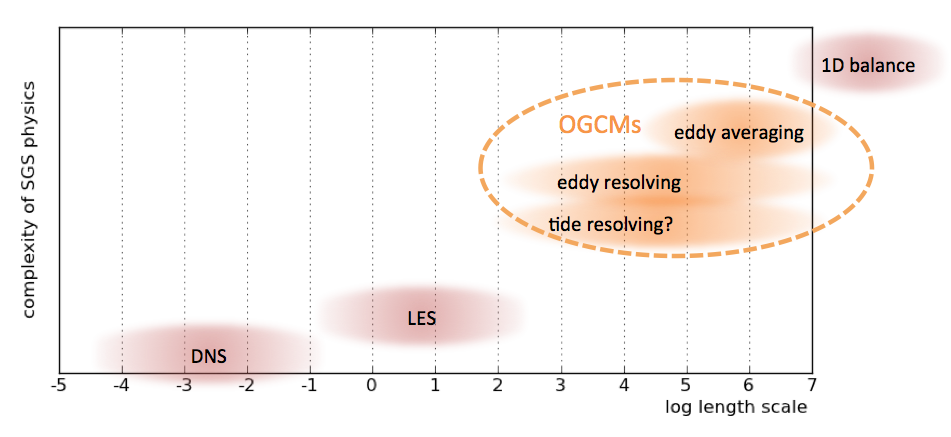
\includegraphics[width=120mm]{figures/images/model_types_schematic.png}
  \caption{Schematic illustration of place of \OGCM{}s in terms of SGS parameterisation of the broad scale range of a turbulent ocean.  For reference, methods from turbulence studies are included: Direct Numerical Simulation and Large Eddy Simulation. Following \citep[fig 5.2]{Petersen:2012tr} and \citep{Stevens:2001kb}.  Inclusion of explicit tides is tentatively placed as a reduction of parameterisation without increased spatial scale resolution.}
  \label{fig:models}
\end{figure}

Common to `big science' simulation practice \citep{Petersen:2012tr} an \OGCM{} embodies a large amount of collective and accumulated programming effort in many lines of computer code; too much for any one person to understand in detail. \\



%-----------------%
\subsection{Ocean observations and data assimilation}
Data assimilation is the framework for combining information from ocean observations and the chaotic dynamics embodied by an \OGCM{}; usefully viewed from a Bayesian perspective\citep{Zaron:2011ft}.\\
Despite the growth of \GOOS{} \citep{Komen:1999ch}, the ocean is fundamentally under-observed for the purposes of physical state estimation.\\


Satellite-based ocean altimetry provides a data stream of special significance to contemporary ocean forecasting \citep{Fu:2001ub}. \\
Derivation of sea level quantities from satellite mounted radar instruments is particularly challenging in shallow water and near coastal boundaries \citep{Woodworth:2011bf}. 
Altimetry has directly enabled contrasting scientific developments in global tides (eg.\citet{Egbert:1996vr},  \citet{Lefevre:2011dg}) and mesoscale ocean variability (eg.  \citet{Wunsch:1998bq}, \citet{Chelton:vi}).

 
% segue into OGCM
%--------------------------------------------------
%--------------------------------------------------
\subsection{Treatment of tides in \OGCM{}s}
\label{S:tides_ogcm}
To date \OGCM{}s in the \GODAE{} heritage have focused on nominally \emph{nontidal} ocean dynamics, with de-tided sea level observations playing a unique role.\\


From that background, recent publications indicate a motivation towards more dynamic representation of the effects of ocean tides.   This is indicative of pervasive goal across numerical simulation practice to increase model concreteness by reducing the role of parameterisations \cite[section 5.3]{Petersen:2012tr}; a reduction of system aggregation \citep{Stevens:2001kb}.\\
Similarly, Griffies describes the ``general trend in ocean climate modelling towards reducing many of the common approximations'' \citep[pp20] {Griffies:2004vs}.
It could be said that the modelling community perceives parameterisations as a compromise that should ideally be replaced with explicit physics when computing power allows.  In spite of this, operational justification is a separate matter.


%-----------------%
\subsection{Nominally non-tidal \OGCM{}s}
\label{S:nontidal}

\BL{} is a nontidal system in that no gravitational body forcing associated with the \ATGP{} is applied.   Subsequently, assimilated observations of sea level are corrected (filtered) using pre-computed global tide models.  The state variable quantifying surface elevation carried by the model is termed sea level anomaly (SLA) which in itself is a rather abstract quantity. Using Stevens' nomenclature, \BL{} simulates an aggregated pseudofluid system with a qualified relationship to the actual ocean.


% split 
Timescales for depth-integrated barotropic and depth-dependant baroclinic ocean state are quite distinct and the design of \OGCM{}s have been influenced by this distinction. \\
%rigid ild
One approach has been to make the so-called `rigid-lid' approximation \cite[pp128]{gill1982atmosphere}. 
The rigid-lid by definition cannot represent explicit barotropic tides, and has other ramifications for ocean forecasting \cite[pp19]{Griffies:2004vs}.\\


% split explicit
A compromise strategy employed in \MOM{} (and other \OGCM{}s) is the so-called `split-explicit' scheme.    
In essence, cheap shallow-water barotropic dynamics are timestepped many times for each relatively expensive update of the full depth-dependant ocean state.  \\
Thus \MOM{} at face value is capable of representing barotropic surface tides.   However, there are several high level arguments against doing so.\\
One reason is the aims to which the model is being employed.  Much of the development of \OGCM{}s has been focused at climate times-scales, tipping the balance of away from the accuracy of high frequency sea level signals.   
Furthermore, in comparison to highly tuned tidal altases, simple and general barotropic can't be expected to achieve similar skill.\\

Filtered altimetry observations provide great value in observing and forecasting mesoscale eddies.
Treating tides as noise is reasonable insofar as the effects on the mesoscale structure are small relative to other source of error.\\

Decomposition of the dynamics into tractable categories for simulation is not aggregation per se, but it certainly does have implications for the role of parameterisations.  \\

From the perspective of \emph{users} of ocean forecasts there is basically no inherent value in decomposition.   
 
%-----------------%
\subsection{Motivation to explicitly resolve tides}

As processing capacity increases, compromises imposed by past computing limitations are re-contextualised.   Inclusion of explicit tides within \OGCM{}s is increasingly affordable from a computational perspective.

With developments to date, exploration of this possibility has been directed primarily at the influence of barotropic tides on the baroclinic structure of the ocean state.   \\


% tides <-> baroclinic
Barotropic tides do interact with the baroclinic structure of the ocean, which conversely impacts the behaviour of barotropic waves and the \emph{non-constant} \citep{Ray:2010jm} nature of tidal constants.\\

Beyond the general simulation goals of model concreteness, it is the possible significance of barotropic/baroclinic interactions for global circulation that provides the primary motivation for considering explicit resolution of tides within \OGCM{}s.   



%-----------------%
\subsubsection{Temporal formulation of tidal forcing}
\label{S:numerical_impl}

The astronomical tidal forcing can be conceptualised as a relatively smooth global surface field that varies in time. 
Perhaps the most significant numerical implementation consideration is how this time variation is formulated.\\


At face value, the \underline{direct formulation} provides the most unmediated and accurate representation of $\eta_{eq}$. Given spherical harmonics $(n,m) \in (2,0) , (2,1) , (2,2)$, the full global tidal forcing can be pre-computed $c_{nm}(t)$ as 6 real valued time series and simple trigonometric functions of location.\\
This approach has the advantage of accurately representing the \ATGP{} and facilitates incorporation of best-practice pre-computed SAL corrections \citep{Egbert:2002ug}. \\
Furthermore, this approach could offer consistent numerical formulation with other barotropic forcing fields.\\


On the other hand, some programatic inconveniences and risks are introduced. 
The input time series must be extracted from the ephemerides at timings to suit each particular simulation.  Furthermore, the extraction process is relatively opaque and would require cross-checks to mitigate the risk of non-fatal errors arising for file dependancies (e.g. incorrect dates).\\
Direct forcing is apparently not as common in the ocean literature as in gravity related studies.   
One instance of forcing a global hydrodynamic model directly is described by Weis and Sunderman \citep{Weis:2008ex} - notably in an non-operational setting.\\\



In contrast, a \underline{harmonic formulation} of $c_{nm}(t)$ for the same range of spatial harmonics requires the specification of many constants for each \emph{temporal} harmonic to be included.  
Hundreds of harmonic components \citep[pp3]{Desai:2006wo} would be required to match the spectral content of an equivilant direct formulation.\\

In practice only a small number (often 8) of the most powerful spectral clusters are specified as `primary constituents'.  
Truncation is based on the relative power of tidal lines within the harmonic development and subsequently requires nodal adjustments (as per Equation \ref{E:Axb}).

Programatically the harmonic approach facilities some attractive simplifications.  
After the specification of a small number of constants, the temporal variation can be cheaply calculated within the ocean model via only a few lines of code.   
For relatively short simulations ($\ll$ 1 year), the nodal corrections are reasonably treated as fixed.   This situation is amenable to de-bugging and has no external dependancies.\\
It is also a relevant consideration that assessment of tidal output is conventionally based on harmonic fits to these same primary constituents.\\

Arbic et al \citep{Arbic:2010us}, apply body forcing using the temporal harmonic representation.  In what appears to be common approach the authors describe developing their implementation via a progressive addition of temporal harmonics: no tides, M2-only, 8 primary constituents.  Treating M2 separately facilitates interpretation and comparison to other literature; including theoretical developments of single frequencies and tidal atlases.



%MOM
The public distribution of \MOM{} includes a very simple module for representing tidal body forcing in a manner suitable for climate simulations\cite[pp263] {Griffies:2008vh}.\\
The eight most powerful constituents (frequency clusters) from $\eta_{eq}$, due to only spherical harmonics $(n,m) = (2,1) , (2,2)$, are written with fixed harmonic amplitude.  SAL is simply parameterised with the scalar approximation. \\
Astronomical phase information is neglected altogether.
Schiller and Feidler \citep{Schiller:2007gk} worked around this gap with addition of a hard-coded astronomical argument offset valid for a particular epoch.\\
Tidal body forcing is written as a depth-independent horizontal term in the momentum equation evolved at the barotropic timestep.
This cheap barotropic code reflects the climate-simulation background of \MOM{}.  
By default, arbitrary forcing terms such as surface fluxes are held constant over iterations of the inner barotropic loop.  
Whilst this is a reasonable optimisation given relatively slow forcing timescales, it is not valid for $\eta_{eq}$ which varies powerfully and quickly.
By employing the temporal harmonic approach to representing the tidal force, $\eta_{eq}$ can be updated algebraically at the barotropic timestep, without requiring relatively expensive file input/output.\\




\subsubsection{Other Aspects of Formulation}
Beyond the basic \ATGP{}, there may be some prospect for translating forcing corrections from \emph{tidal} data assimilation models to an \OGCM{}. \\
The \underline{Generalised Inverse} (GI) \cite[pp345] {Zaron:2011ft} approach employed by \OTIS{} \cite{Egbert:2002ug}, draws an objective trade-off between observational and dynamic uncertainties; the ``inevitably approximate nature of the discretised dynamical constraints''\cite[pp155]{Egbert:1996vr}.  The inversion process involves determining adjusted forcing to achieve the optimal trade off.\\
Thus it is speculated that complementary use of \OTIS{} may be exploited to improve the representation of a stationary tidal signal in the time-stepping \OGCM{}.  \\


%OBC
Application of tidal forcing to a \emph{regional} prediction system raises the topic of open boundary conditions (\obc{}).  \obc{}s are of fundamental importance for limited area ocean models but review is considered beyond the scope of this document at present.\\


%-----------------%
\subsubsection{Vertical Mixing}

% climate mixing
An emphasis on improving the representation of \emph{baroclinic} circulation is apparent in \OGCM{} simulations implementing explicit tides.\\
Simmons et al \citep{Simmons:2004fi} are motivated to increase the concreteness of parameterisations with regard to the conversion of barotropic tidal energy.  Surface elevations were not the target of these simulations. \\


% schiller MOM
At timescales closer to those of operational forecasts, Schiller et al have also employed explicit tides within free-surface configurations of \MOM{}.  
Better representation of baroclinic mixing is again a primary motivation. 
Specifically, improved understanding of water mass structures \cite{Schiller:2004fv} and upper ocean circulation \cite{Schiller:2007gk} were cited as justifications for the implemention.  
Whilst the resolution of these configurations did not aim to resolve internal tide processes, explicit barotropic tidal currents enabled vertical mixing parameterisations to reflect spatially and temporally varying tidal effects.\\
In addition to the focus on mixing, surface level skill was evaluated against a coastal tide gauge and shown to offer some promise as a prognostic output \citep[Fig 2]{Schiller:2007gk} - apparently despite expectations.   
The issue of top-layer thickness limitations on surface elevation magnitudes highlighted by the authors does not directly apply to the contemporary \BL{} configuration of \MOM{}, which employs the $z^*$ coordinate \citep{Brassington:2012wm}.\\


%-----------------%
\subsubsection{Conversion Parameterisation}

% wave drag
Bringing astronomical forcing effects from `parameterised' to 'resolved' is a significant change with ramifications for parameterisation settings generally. \OGCM{}s parameterisation typically do not scale well.\\



Arbic et al \cite{Arbic:2004wz} discuss the `inordinately large' bottom drag values required by hydrodynamic tidal models and argue for the value of additional topography-based parameterisations.   
For example, the wave drag scheme described by Jayne \cite{Jayne:2001tr} is designed to spatially align barotropic dissipation over features such as mid-ocean ridges that are known to be source of internal tide generation.  Whilst a spatial concentration over internal tide generation locations is attractive - the relationship to vertical mixing may be misaligned to the extent that the energy cascade is non-local.  Internal wave propagation has a frequency/latitude dependance, with a qualitative transition from propagating to trapped occurring poleward of critical latitudes.  Furthermore `` the extent to which internal tides produce turbulence as they propagate away from their generation sites is not clear'' \citep[pp812]{Jayne:2001tr}.\\



It is notable that a related scheme is employed by the operational \emph{non-tidal} barotropic model employed for altimetry corrections (T-UGO, previously MOG2D)\citep{Carrere:2003cj}.  Model parameters, including a `internal wave' term, were tuned by means of a tidal simulation and comparison to tidal harmonics. \\


% schiller drag
The need to apply a special dissipation term to barotropic tides is also described by Schiller \citep[Eq 6]{Schiller:2007gk}.   This additional drag term was applied only within the barotropic loop and was designed via a tuning procedure but not described in detail.



% Arbic HYCOM
Arguably the leading tidal \OGCM{} developments described in the literature are those of Arbic et al. who have implemented a tidal version of HYCOM \cite{Arbic:2005gv,Arbic:2009hf,Arbic:2010us,Arbic:hy}.\\
Generally, the development procedure described involves a preliminary tuning of a spatially varying wave drag term.  Tuning is achieved on the basis of minimising the disagreement between a M2-only simulation and a published tidal atlas.   
Temporal filtering measures are described to isolate the action of the wave drag term from inappropriate application to other dynamics.  \\
At face value, the use of a parameterisation for baroclinic tide conversion in a full baroclinic model appears somewhat inconsistent.   The justification offered by authors is based on the spatial resolution of the model compared to theoretical expectations of internal tide wavelengths:
\noindent \begin{quotation}
$\dots{}$  vertical mode numbers beyond about 10 are probably not resolved at all in the simulations $\dots{}$, and vertical mode numbers beyond one or two are probably not well-resolved. Thus horizontal resolution limitations are in part responsible for the fact that parameterised topographic wave drag is still required to achieve accurate barotropic tides in baroclinic tide models. \citep[pp177]{Arbic:2010us}
\end{quotation}



%-----------------%
\subsection{Coastal boundaries}

The impact of lateral boundaries and shallow water effects on representing global tides is a topic that arises in time-stepped forward models.\\
In a barotropic simulation forced directly by tidal ephemerides \cite{Weis:2008ex}, the authors indicate that solutions for \emph{deep-water} partial tides are significantly influenced by the explicit simulation of broad-band tidal spectrum.   
(It is notable that this simulation did not include a `wave drag' term - but the authors sicte this exclusion as a likely source of error \citep[pp5]{Weis:2008ex})\\
Based on a more thorough and analytical approach, Arbic et al investigations provide a similar conclusion:
\noindent \begin{quotation}
$\dots{}$ the back-effect of coastal tides upon open-ocean tides is demonstrated in numerical experiments in which removal of regions of resonant coastal tides significantly alters tidal amplitudes (generally, increasing them) and phases, over basin-wide and even global scales.\citep[pp263]{Arbic:2009in}
\end{quotation}

With regard to operational \OGCM{}s these discussions are taken to highlight the potential impact of lateral conditions designed for nontidal simulations.  
One instance are the so-called `earth-works', where bathymetry and coastlines are manually adjusted in the interest of allowing certain ocean circulation features to exist.  
Similarly relevant is the representation of barotropic dissipation in shelf regions. 
Specific cases that may have an impact on the Australian coastline include the parameterisation of bottom dissipation over the Great Barrier Reef, and possibly the geometry of coastline features such as the Gulf of St Vincent and King Sound.




% DA
Inclusion of explicit tides within an \OGCM{} thus offers the potential to improve the simulation of the global ocean state, but in doing so introduces many novel challenges.\\
How to approach data assimilation is particularly problematic.  Assimilation of corrected observations and the exclusion of tidal dynamics provides has been more or less fundamental to the design of the current generation of \GODAE{} systems (Section \ref{S:nontidal}).\\
Sea level observations provide a powerful constraint upon operational ocean models, and how to assimilate sea level into models that dynamically include both mesoscale and tidal motions is an open question.   Maintaining the conceptual split between periodic and aperiodic motions appears to be a reasonable general framework.

